One of the perks of a (semi-)Bayesian approach to regression modelling is that we are able to use Bayesian post-estimation machinery involving the relevant posterior distributions.
With the normal I-prior model, there is the added benefit that posterior distributions are easily obtained in closed form.
The plots that are shown in this subsection is a continuation of the example from \autoref{sec:compareestimation}.

Recall that for the I-prior model \cref{eq:model2}, the regression function $f(x) = \sum_{i=1}^n h_{\hat\eta}(x,x_i)\tilde w_i$
%, where $\hat\eta$ is the ML estimate for the kernel parameters, 
has the posterior Gaussian distribution specified by the  multivariate-normal mean and variance of the $\tilde w_i$'s given in \cref{eq:posteriorw}.
Denote by $\bh_{\hat\eta}(x)$ the $n$-vector with entries equal to $h_{\hat\eta}(x,x_i)$.
Precisely, the posterior density for the regression function is
\begin{align}
  p\big(f(x) | \by \big) \sim \N \Big( 
  \bh_{\hat\eta}(x)\hat\bw, 
  \bh_{\hat\eta}(x)^\top \big(\bH_{\hat\eta}\hat\bPsi\bH_{\hat\eta} + \hat\bPsi^{-1}\big)^{-1} \bh_{\hat\eta}(x) 
  \Big)
\end{align}
for any $x$ in the domain of the regression function.
Here, the hats on the parameters indicate the use of the optimised model parameters, i.e. the ML or MAP estimates.

\begin{figure}[p]
  \centering
  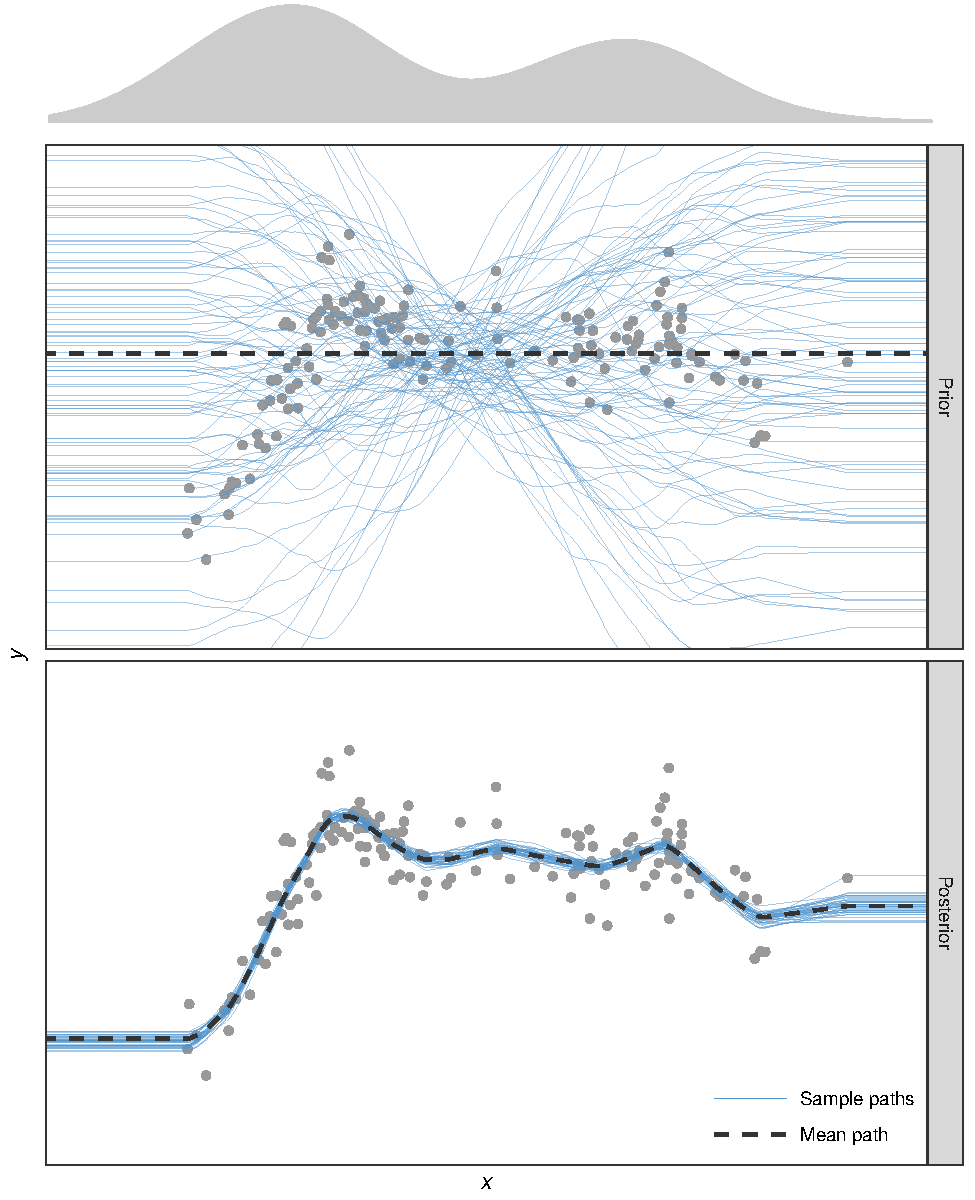
\includegraphics[width=0.95\textwidth]{figure/04-post_reg_prior_post}
  \caption[Prior and posterior sample path realisations]{Prior (top) and posterior (bottom) sample path realisations of regression functions drawn from their respective distributions when $\cF$ is a fBm-0.5 RKHS. At the very top of the figure, a smoothed density estimate of the $x$'s is overlaid. In regions with few data points (near the centre), there is little Fisher information, and hence a conservative prior closer to zero, the prior mean, for this region.}
\end{figure}

Prediction of a new data point is also of interest.
A priori, assume that $y_\new = \hat\alpha + f(x_\new) + \epsilon_\new$, where $\epsilon_\new \sim \N(0,\psi^{-1}_\new)$, and $f\sim \text{I-prior}$.
Denote the covariance between $\epsilon_\new$ and $\bepsilon = (\epsilon_1,\dots,\epsilon_n)^\top$ by $\bsigma_\new^\top \in \bbR^n$.
Under an iid model (assumption \ref{ass:A3}), then $\psi_\new = \psi = \Var \epsilon_i$ for any $i\in\{1,\dots,n\}$, and $\bsigma_\new^\top=\bzero$, but otherwise, these extra parameters need to be dealt with somehow, either by specifying them a priori or estimating them again, which seems excessive.
In any case, using a linearity argument, the posterior distribution for $y_\new$ is normal, with mean and variance given by
\begin{gather}
  \E[y_\new|\by] = \hat\alpha + \E \big[ f(x_\new) |\by \big] + \text{correction term} \\
  \text{and} \nonumber \\
  \Var[y_\new|\by] 
  = \Var\big[f(x_\new)|\by\big] + \psi^{-1}_\new + \text{correction term}.
\end{gather}
A derivation is presented in \autoref{apx:postpred}.
Note, that the mean and variance correction term vanishes under an iid assumption \ref{ass:A3}.
The posterior distribution for $y_\new$ can be used in several ways. 
Among them, is to construct a $100(1 - \alpha)\%$ credibility interval for the (mean) predicted value $y_\new$ using
\[
  \E[y_\new|\by] \pm \Phi^{-1}(1 - \alpha/2) \cdot \Var[y_\new|\by]^{\half},
\]
where $\Phi(\cdot)$ is the standard normal cumulative distribution function.
One could also perform a posterior predictive density check of the data $\by$, by repeatedly sampling $n$ points from its posterior distribution.
This provides a visual check of whether there are any systematic deviances between what the model predicts, and what is observed from the data.

\begin{figure}[p]
  \centering
  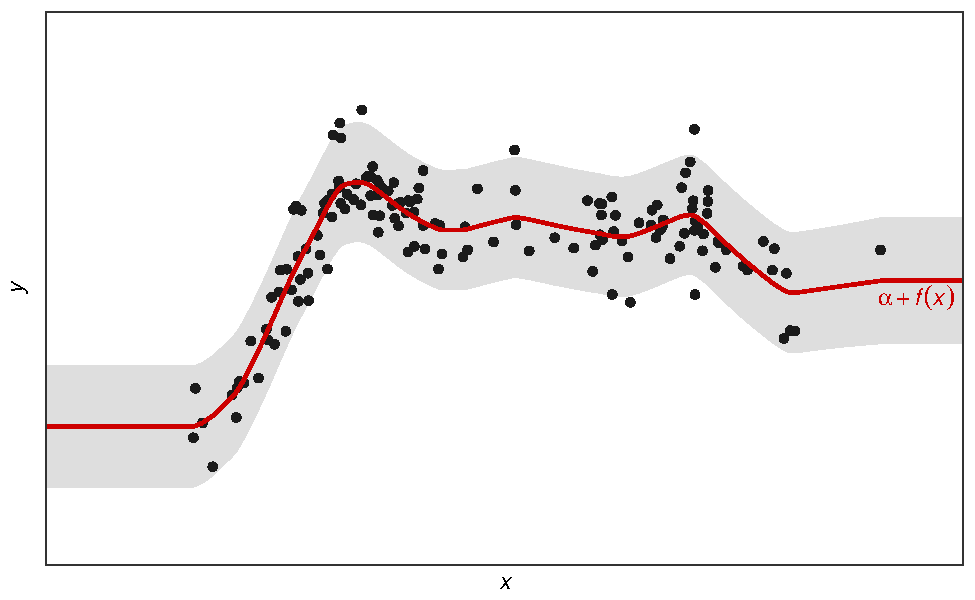
\includegraphics[width=0.9\textwidth]{figure/04-post_reg_cred}
  \caption{The estimated regression line (solid black) is the posterior mean estimate of the regression function (shifted by the intercept), which also gives the posterior mean estimate for the responses $y$. The shaded region is the 95\% credibility interval for predictions. The true regression line (dashed red) is shown for comparison.}
  \vspace{1em}
  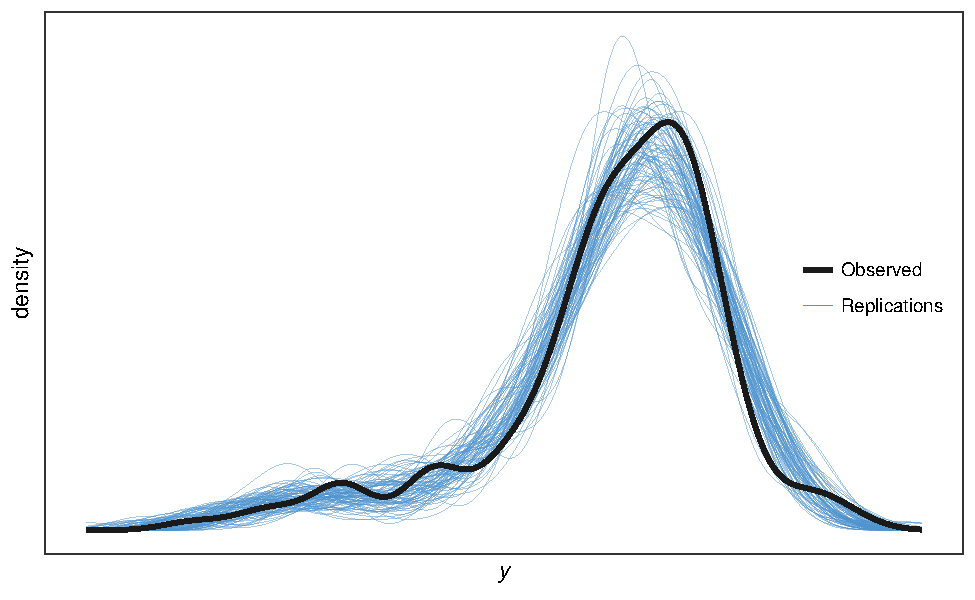
\includegraphics[width=0.9\textwidth]{figure/04-post_reg_ppc}
  \caption{Posterior predictive density checks of the responses: repeated sampling from the posterior density of the $y_i$'s and plotting their densities allows us to compare model predictions against observed samples.}
\end{figure}

Lastly, we discuss model comparison.
Recall that the marginal distribution for $\by$ after integrating out the I-prior for $f$ in model \cref{eq:model2} is a normal distribution.
Suppose that we are interested in comparing two candidate models $M_1$ and $M_2$, each with the parameter set $\theta_1$ and $\theta_2$.
Commonly, we would like to test whether or not particular terms in the ANOVA RKKS are significant contributors in explaining the relationship between the responses and predictors.
A log-likelihood comparison is possible using an asymptotic chi-squared distribution, with degrees of freedom equal to the difference between the number of parameters in $\theta_2$ and $\theta_1$.
This is assuming model $M_1$ is nested within $M_2$, which is the case for ANOVA-type constructions.
Note that if two models have the same number of parameters, then the model with the higher likelihood is preferred.

\begin{remark}
  This method of comparing marginal likelihoods can be seen as Bayesian model selection using \emph{empirical Bayes factors}, where the Bayes factor of comparing model $M_1$ to model $M_2$ is defined as
  \[
    \BF(M_1,M_2) = \frac{\int p(\by|\theta_1,\bff)p(\bff) \dint \bff }{\int p(\by|\theta_2,\bff)p(\bff) \dint \bff}.
  \]
  The word ‘empirical’ stems from the fact that the parameters are estimated via an empirical Bayes approach (maximum marginal likelihood).
  This approach is fine when the number of comparisons to be made is small, but can be computationally unfeasible when many marginal likelihoods need to be pairwise compared.
  In Chapter 6, we explore a fully Bayesian approach to explore the entire model space for the special case of linear models.
\end{remark}
